\documentclass[12pt]{article}
% \documentclass[conference]{IEEEtran}

% Packages
% Packages

% \usepackage{fancyhdr} % Required for custom headers
% \usepackage{lastpage} % Required to determine the last page for the footer
% \usepackage{extramarks} % Required for headers and footers
% \usepackage[usenames,dvipsnames]{color} % Required for custom colors
\usepackage{graphicx} % Required to insert images
% \usepackage{listings} % Required for insertion of code
% \usepackage{courier} % Required for the courier font
% \usepackage{dsfont} % For special math characters
% \usepackage{verbatim}

%\usepackage{amsmath, amssymb, bm} % For matrix notation
\usepackage[english]{babel}
\usepackage[paperwidth=8.5in,paperheight=11in,margin=1.0in]{geometry}
\usepackage{listings}
\usepackage{hyperref}
%\usepackage[cmex10]{amsmath, bm}
\usepackage{amsmath, bm}
\usepackage{blkarray}








% formatting
\pdfcompresslevel0

\lstset{ columns=flexible, breaklines=true, basicstyle=\small\ttfamily}
\setcounter{MaxMatrixCols}{20}
\linespread{1.3} %1.5x line spacing




\begin{document}
\title{Predicting Salaries From Job Descriptions}

\author{
Elijah Bernstein-Cooper, Ben Conrad, Ahmed Saif
}
\maketitle

%NB: Double ticks do not work for apostrophes, look at the output before changing all.  They do work for the first quotation mark.


% ------------------------------------------------------------------------------
\section{Introduction}
% ------------------------------------------------------------------------------

    Under the context of natural language processing, this lab explores the
    relation between job descriptions and salaries.  This topic was the focus
    of a \href{http://www.kaggle.com/c/job-salary-prediction}{Kaggle}
    competition whose sponsor, Adzuna, had a database of job listings of which
    only half provided salary information (the winner received \$3000).  As
    applicants will more likely apply to descriptions that give a salary,
    Adzuna's placement rate (and hence revenue) is improved if they can provide
    an estimated salary for those descriptions that did not originally include
    one. The employee recruiting business is structured so that Adzuna
    generally can't directly ask the companies to provide salary estimates.
    This is challenging from the legal standpoint, as grossly incorrect
    salaries may expose Adzuna to claims from applicants and companies, and
    applicant experience, since Adzuna's estimates must seem plausible to
    applicants before they will be willing to spend the time applying.

    While Adzuna could manually estimate these salaries, scalability encourages
    throwing computers at the problem.  In this lab we will be using Adzuna's
    job description and salary datasets, divided into training and test sets.
    These descriptions vary in word count, industry, employment level, and
    company location, while the salaries are the mean of the provided salary
    range.  The variability in description content leads to notoriously sparse
    matrices, so we will be interested in the tradeoffs of various feature
    descriptors.  The naive approach to this problem is to count the
    occurrences of individual words and associate them to salaries; here each
    word is a feature and as there are many descriptive words the resulting
    matrices will be sparse.  Other feature choices may be individual word
    length, occurrences of word pairs or triplets (ie ``technical
    communication``), n-grams (sequences of n characters), and many others. It
    is common to ignore stop words like ``the",``a",``it",``you",``we", etc.
    because they add little information.

% ------------------------------------------------------------------------------
\section{Warm-Up}
% ------------------------------------------------------------------------------

    Our goal in the warm-up is to use two job descriptions with known
    salaries to predict the salary of another job given the description. Here
    are two examples from the dataset: 
    
    \begin{lstlisting}

        Engineering Systems Analyst Dorking Surrey Salary ****K Our client is
        located in Dorking, Surrey and are looking for Engineering Systems
        Analyst our client provides specialist software development Keywords
        Mathematical Modelling, Risk Analysis, System Modelling, Optimisation,
        MISER, PIONEEER Engineering Systems Analyst Dorking Surrey Salary ****K

    \end{lstlisting}

    with a salary of \$25,000 and 

    \begin{lstlisting}

        A subsea engineering company is looking for an experienced Subsea Cable
        Engineer who will be responsible for providing all issues related to
        cables. They will need someone who has at least 1015 years of subsea
        cable engineering experience with significant experience within
        offshore oil and gas industries. The qualified candidate will be
        responsible for developing new modelling methods for FEA and CFD. You
        will also be providing technical leadership to all staff therefore you
        must be an expert in problem solving and risk assessments. You must
        also be proactive and must have strong interpersonal skills. You must
        be a Chartered Engineer or working towards it the qualification. The
        company offers an extremely competitive salary, health care plan,
        training, professional membership sponsorship, and relocation package
    
    \end{lstlisting} having a salary of \$85,000.

    One method to predict the salary from another description is least squares
    estimation.  Least squares estimation can be thought of as an optimization
    problem which aims to minimize the error estimated and measured data.  In
    our case, we want to predict salaries from the words contained in the job
    descriptions.  For now, let's consider only occurrences of ``analyse" in
    the description.  If you plot the number of occurrences against the job
    salary, you might produce something like
    
    \begin{center}
    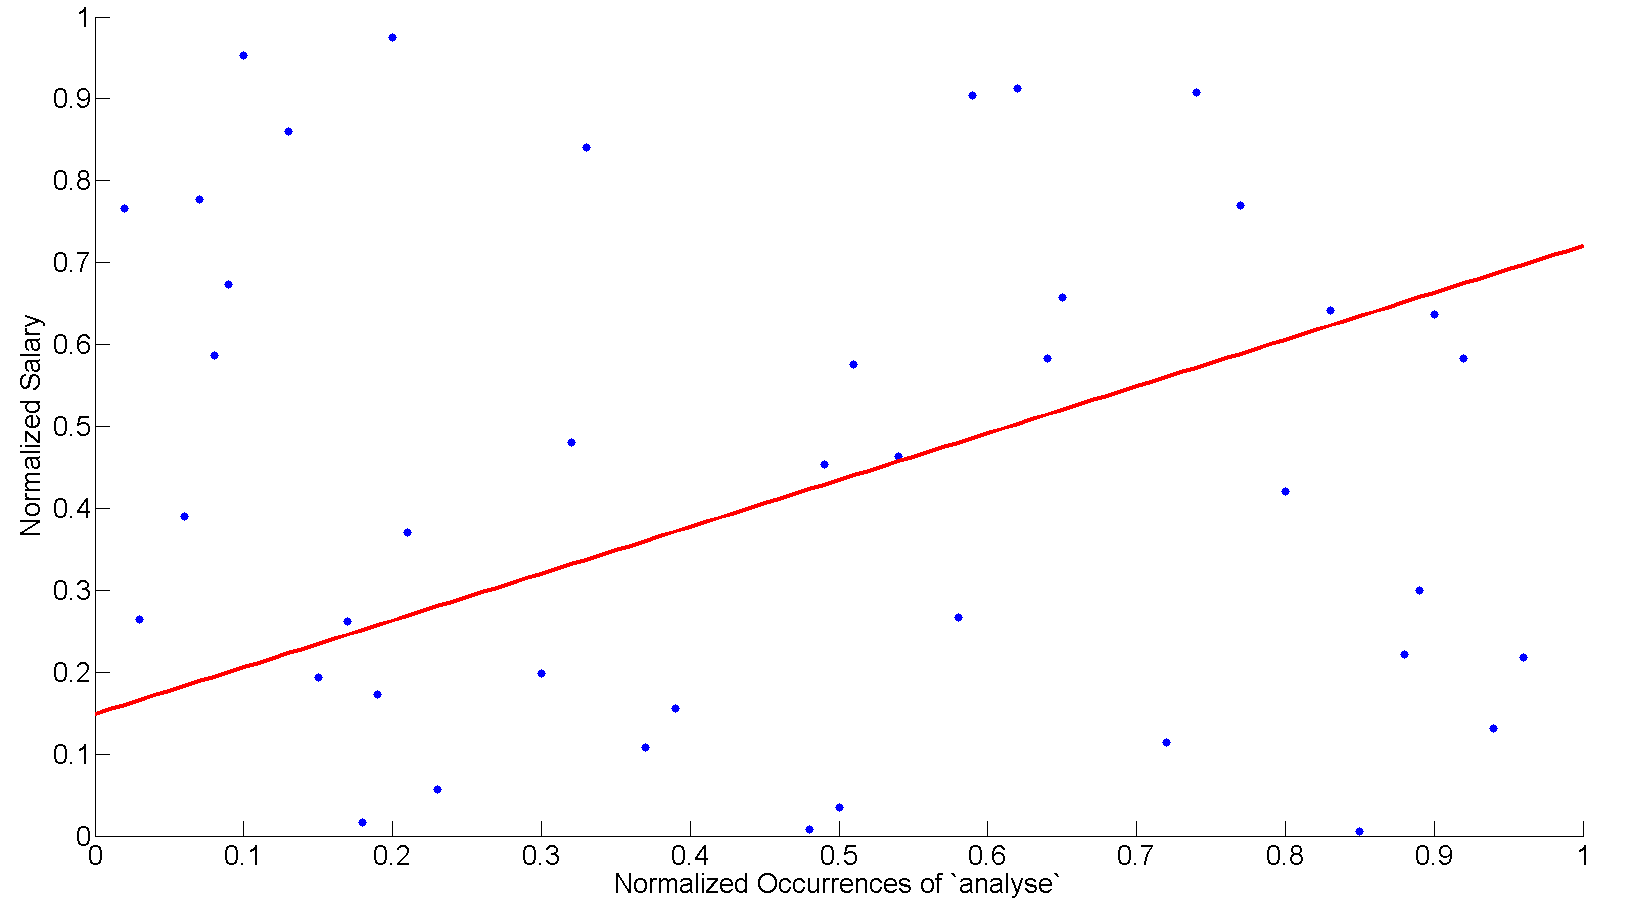
\includegraphics[width=\linewidth]{figLSE}
    \end{center}
    
    In solving the least squared problem, we're looking for the line which
    passes nearest to all of the points, as measured by the Euclidean distance,
    or

    \begin{equation}
    error = \sqrt{ (x_i - x_L)^2 + (y_i - y_L)^2} 
    \end{equation}
 
    If we considered two words, say ``analyse" and ``qualified", we would now
    have a 3D space to find our least squared solution with one axis being
    occurrences of ``analyse," another ``qualified," and the third the salary.
    Here, our solution will be a plane that slices the 3D space; adding more
    words - or features as they're more generally described - increases the
    dimensionality of this space, and our solution becomes a hyperplane.  In
    all cases, we want to minimize the distance from all of the data points to
    the lower-dimensional estimate.
    
    We would like to determine the words that best predict salary, or even
    better the frequency of the words which best predict salary. Here we show
    the 11 most common words for each description:

    \begin{center}
    \begin{minipage}[t]{.4\textwidth}
    Description 1
    \newline
    \newline
        \begin{tabular}{l|c}
            ****k & 2 \\
            analysis & 1\\
            analyst & 3\\
            and & 1\\
            are & 1\\
            client & 2\\
            development & 1\\
            dorking & 3\\
            engineering & 3\\
            for & 1\\
            in & 1
        \end{tabular}
    \end{minipage}
    \begin{minipage}[t]{.4\textwidth}
    Description 2
    \newline
    \newline
        \begin{tabular}{l|c}
            1015 & 1 \\
            a & 2 \\
            all & 2 \\
            also & 2\\
            an & 3 \\
            and & 5 \\
            assessments & 1 \\
            at & 1 \\
            be & 6 \\
            cable & 2 \\
            cables & 1
        \end{tabular}
    \end{minipage}
    \end{center}

    We can collect these word counts into the matrix $\bm{A}$, and the salaries
    into the vector $\bm{b}$. $\bm{A}$ will have 2 rows, one for each
    description and as many columns as there are unique words between the two
    descriptions. $\bm{b}$ will have 2 rows, one salary for each description,
    and one column. $\bm{A}$ and $\bm{b}$ will look like the following

    \begin{equation*}
        \bm{A} = 
        \begin{bmatrix}
           2 & 0 & 0 & 0 & 0 & 0 & 1 & 3 & 1 & 1\cdots\\
	0 & 1 & 2 & 2 & 2 & 3 & 0 & 0 & 5 & 0\cdots
        \end{bmatrix}
    \end{equation*}
	
    \begin{equation*}
        \bm{b} = 
        \begin{bmatrix}
        2500\\
        85000
        \end{bmatrix}
    \end{equation*}

    with the first two corresponding to the two occurrences of `****k' in the first descripton and the later 1, 5 column to occurrences of `and' in both descriptions.


    We can then set up our problem as 
    \begin{equation}\label{eq:linsolve}
        \bm{b} = \bm{Ax}
    \end{equation}

    \noindent where $\bm{x}$ contains the weights (importance) of each word in
    predicting the salary of the job. We can find a solution for $\bm{x}$,
    $\bm{\hat{x}}$, by minimizing the residual errors between $\bm{b}$ and
    $\bm{Ax}$.  This is the same as minimizing the sum of squared residuals,

    \begin{equation}
        \|\bm{b} - \bm{Ax}\|^2_2
    \end{equation}

    \noindent This optimization has a well-known solution for $\bm{\hat{x}}$
    \begin{equation}
        \bm{\hat{x}} = (\bm{A}^{T}\bm{A})^{-1}\bm{A}^T\bm{b}
    \end{equation}

    when $\bm{A}$ is positive semidefinite, or rather, invertible.
    
    In cases when $\bm{A}$ is not positive semidefinite, as in the $\bm{A}$
    derived from the word counts above, we can use the right psuedo-inverse of
    $\bm{A}$.  In Matlab this is 
    
    \begin{equation} 
        \bm{\hat{x}} = \texttt{pinv}(\bm{A})*\bm{b}
        % I don't want to introduce the svd in the warmup, but the inverse does
        %not work...  
    \end{equation}

    Using the solution for $\bm{\hat{x}}$, our least-squares solution to this
    problem, $\bm{\hat{x}}$ is:

    \begin{equation*}
        \bm{\hat{x}} = 
        \begin{blockarray}{[c] l}
            1819.6517 & ``be"           \text{ from } [0, 6] \\
            1730.9558 & ``and"          \text{ from } [1, 5] \\
            1427.6805 & ``for"          \text{ from } [1, 4] \\
            1250.2887 & ``engineering"  \text{ from } [3, 2] \\
            1213.1011 & ``must"         \text{ from } [0, 4] \\
            1213.1011 & ``will"         \text{ from } [0, 4] \\
            1213.1011 & ``you"          \text{ from } [0, 4] \\
            909.8258 & ``an"            \text{ from } [0, 3] \\
            909.8258 & ``subsea"        \text{ from } [0, 3] \\
            909.8258 & ``the"           \text{ from } [0, 3] \\
            732.4341 & ``modelling"     \text{ from } [2, 1] \\
            \vdots & \hspace{1cm}\vdots
        \end{blockarray}
    \end{equation*}

    The bracketed numbers give the number of occurrences of that word in each
    of the descriptions; with only two samples it should not be surprising that
    the most heavily-weighted words are unique to each description.  But notice
    how some words are identically-weighted and that from these 11 `most
    important' words, none of them are highly descriptive.
    
    % --------------------------------------------------------------------------
    % Activity 
    % --------------------------------------------------------------------------
    \begin{center} 
        
        \fbox{\begin{minipage}{40em} {\bf \large Activity 1} \\ Construct the
                above $\bm{A}$ and $\bm{b}$ matrices using the 1$^{\rm st}$ and
                2$^{\rm nd}$ descriptions in the warm-up data,
                warmup\_train.mat. $\bm{A}$ should be a 2$\times m$ matrix
                where $m$ is the number of unique words between the two
                descriptions.  $\bm{b}$ should be a 2$\times$1 matrix. Can you
                reproduce the above solution for $\bm{\hat{x}}$? Report on the
                uniqueness of the solution for $\bm{\hat{x}}$ in this problem.
                Support your conclusion.\\
            
            The following commands may be helpful:
            \begin{center}
                \texttt{word = strrep(`word',`charactersToReplace',`replaceThemWith')} \\
                \texttt{parts = strsplit('sentence')}\\
                \texttt{lowercase = lower('UpperCase')}\\
                \texttt{uwords = unique(wordArray)}\\
                \texttt{sortedArray = sort(unsortedArray)}\\
            \end{center}
            \end{minipage}
        }
        
    \end{center}
    % --------------------------------------------------------------------------
    % --------------------------------------------------------------------------
    
    Next we wish to predict the salary of another description using our
    $\bm{\hat{x}}$. 

    \begin{lstlisting}
        Our client is part of an international hotel chain that require an
        experienced Cluster Revenue Manager to be based in Hertfordshire. The
        Cluster Revenue Manager will drive and influence revenue for three to
        four hotels. As Cluster Revenue Manager you will maximise revenue,
        market share and profits for multiple hotels through the strategic
        coordination of revenue management processes and procedures. The
        Cluster Revenue Manager will drive the continued development and growth
        of customer service standards, revenue and profits from multiple hotels
        and to deliver the company’s mission relating to profit, people,
        customer and quality. You will currently be a Cluster Revenue Manager
        or a Regional/ Area Revenue Manager looking after a minimum of two
        propertys or a Revenue Manager in a large unit managing both rooms and
        conference space. This job was originally posted as
        www.caterer.com/JobSeeking/ClusterRevenueManager_job****
    \end{lstlisting} having a salary of \$45,000.
    
    % --------------------------------------------------------------------------
    % Activity 
    % --------------------------------------------------------------------------
    \begin{center} 
        
        \fbox{\begin{minipage}{30em}

            {\bf \large Activity 2} \\
            Use your solution for $\bm{\hat{x}}$ in Activity 1 to estimate the
            salary of the third description in the warm-up test data,
            warmup\_test.mat.  Since $\bm{\hat{x}}$ is a weighting of words
            from the first two descriptions, ignore any words that are unique
            to the third description.
            \end{minipage}
        }
        
    \end{center}
    % --------------------------------------------------------------------------
    % --------------------------------------------------------------------------

    We now construct the matrix $\bm{A}$ for this description. This matrix will
    only contain frequencies of words that were present in the previous two
    descriptions, so many words in this new description will be left out. We
    can then use our weights for best predicting words, $\bm{\hat{x}}$ to
    estimate the salary of the job for this new description, now contained in
    the matrix $\bm{b}$. Our estimated salary will be stored in $\bm{\hat{b}}$,
    which we estimate from Equation~\ref{eq:linsolve}. \\

    The estimated salary is \$3032.80. About \$41,967 different from the true
    salary associated with the job. Would Adzuna likely use this technique of
    linear least squares? Consider how populated our $\bm{A}$ matrix is for the
    third description. Is the matrix well-populated or sparsely-populated?
    Based on your intuition, are all of the words in $\bm{\hat{x}}$ likely to
    be good predictors of salary? How might paring down the keywords in our
    data matrix benefit us? In the following sections we will introduce ways to
    include many more descriptions in our analysis, and derive more accurate
    predictors of a salary based on the description.

\section{Feature Descriptors / Regularized LS - Elijah}
About a page...
Have them solve a 10 description problem w/ and w/o regularization?

\section{The Lasso Method - Ahmed}
Describe Lasso briefly, that it's a regularized method which 'works better' for this sparse problem..
Solve same 10 problem with Lasso
Provide A, A inv, and xhat for a larger problem?

\section{Using the Results...Ben}

%Ok, now let's turn it around:
%We've computed which words employers use to indicate high salaries, can we use this to advise applicants what salary their resume is applying for.



\section{Conclusion}

\end{document}




